% !TEX encoding = UTF-8
% !TEX program = lualatex

\documentclass[a4paper]{article}

\usepackage[left=1.5cm, right=1.5cm, top=1cm, bottom=2cm]{geometry}

\usepackage{mathtools, amssymb}
    \def\RR{\mathbf R}
    \def\CC{\mathbf C}

\usepackage[no-math]{fontspec}
    \setmainfont{Noto Serif}
    \setsansfont{Noto Sans TC}
    \setmonofont{Noto Sans Mono}

\usepackage{tikz}

\begin{document}

\parindent 0pt
\parskip 1em

\newcounter{p}\newcounter{c}\def\Problem{\stepcounter{p}[\thep] }
\def\choice{\stepcounter c\ifnum\value c=27\setcounter c1\fi(\Alph c) }
    
\section*{Complex Variable - Final Exam}

\sffamily

考試時間 Test time 10:30:00 am to 12:00:00 pm; 1.5 hours.
以教室投影機時鐘為準 Using the projected clock.
用空白紙張作答 Answer on blank paper.
每個問號一分 One point per question mark.
全對才給分 No partial credit.
可以帶 991 You can use fx-991 or anything weaker.
舉手問問題 Raise your hand to ask questions.

\rmfamily

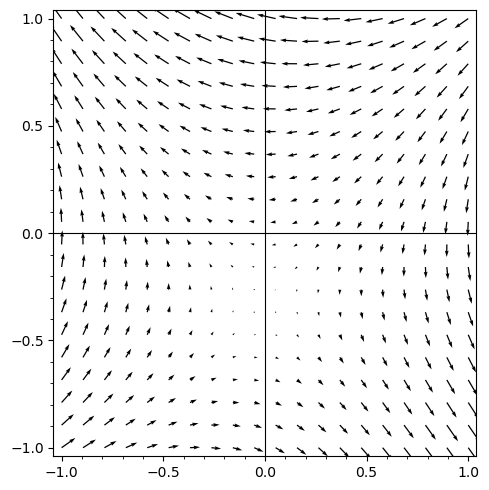
\includegraphics[height=5cm]{f1.png}
\\[-5.5cm]

\hangindent=5.5cm \hangafter=-11
\Problem
Consider the vector field to the left.
When $x > 0$, its divergence is?
\choice $> 0$
\choice $= 0$
\choice $< 0$
\\~\\
\Problem
When $y < 0$, its curl is?
\choice $> 0$
\choice $= 0$
\choice $< 0$
\\~\\
\Problem
Which of the following is the most probable source of this vector field?
\choice heat flow that has reached steady state
\choice fluid flow that hasn't reached steady state
\choice electric field with positive charge density
\choice magnetic field generated by current flowing into your eyes
\\~\\
\Problem
Among the points $m/3 + ni/3$ where $m, n$ are integers,
Which point is closest to a zero of the vector field?
\\~\\
\Problem
$F = (P, Q)$ is curl-free and divergence-free.
Which of the following are holomorphic?
\choice $P + Qi$
\choice $P - Qi$
\choice $(P + Q) + (P - Q)i$
\choice $(P + Q) - (P - Q)i$

\Problem
$i^{i^{i^i}} = 0.0500922361093212 + 0.6?2?1?527036004i$.

\Problem
$\log_2(2^{60} + 123 + 2^{60}i + 456i)
= 60.5000000000000003?2?6?489396 + 1.1330900354567986607547773322i$.

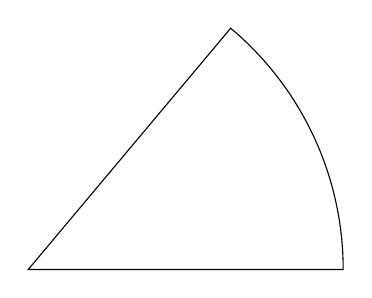
\begin{tikzpicture}
    \draw (0, 0) -- (4, 0) arc (0:50:4) -- cycle;
\end{tikzpicture}
\\[-4cm]

\hangindent=4.5cm \hangafter=-8
\Problem
What is the symbolic result of this integral
$\int_0^\infty (x^4 + x^6) / (x^{12} + 1) \, dx$?
Hint: consider contour integral with a domain like the one to the left.
\\~\\
\Problem
What is the Mobius map $\mu$ that maps
$-2, -1, \infty$ to $-1, \infty, -2$, respectively?
\\~\\
\Problem
What is the only point $d \in \CC$ in the upper half plane
such that $\mu(d) = d$?
\\~\\
\Problem
Recall that $\Delta(z) = \int _0^z (x + 1)^{-2/3} (x + 2)^{-2/3} \, dx$
maps the upper half plane to a mystery triangle.
Let $\rho$ be the rotation that rotates the mystery triangle
by $120$ degrees CCW about its center.
We see that
\[
    \Delta(\mu(-2)) = \Delta(-1) = \rho(\Delta(-2)), \qquad 
    \Delta(\mu(-1)) = \Delta(\infty) = \rho(\Delta(-1)), \qquad 
    \Delta(\mu(\infty)) = \Delta(-2) = \rho(\Delta(\infty))
\]
So $\Delta^{-1}(\rho(\Delta(\bullet)))$ is a map that maps ? to itself
and coincide with $\mu$ at three points.
Does it necessarily imply that $\Delta^{-1}(\rho(\Delta(\bullet))) = \mu$?
If there are at least two maps that coincide with $\mu$
at three points, describe one more such map.
If there is only one such map,
tell me the title of the lecture note that contains the proof idea.

\Problem
I checked and $\Delta^{-1}(\rho(\Delta(\bullet)))$ is indeed equal to $\mu$,
what is the center of the mystery triangle?
Describe the point symbolically using variables introduced so far.

\Problem
According to Schwarz--Christoffel formula,
$\diamondsuit(z) = \int _0^z ((x^2 - 1) (x^2 - k))^{-1/2} \, dx$
maps the upper half plane to a pentagon
with four $90^\circ$ angles and one $180^\circ$ angle.
So it is equivalent to saying that
it maps the upper half plane to a rectangle.
What is the value of $k > 0$ such that the image
is not just a rectangle but actually a square?
Hint: if it is a square, it can be rotated using Mobius maps.

\Problem
According to Schwarz--Christoffel formula,
$\Lambda(z) = \int _0^z (x^2 - 1)^{-3/4} \, dx$
maps the upper half plane to a right triangle.
What is the length of the hypotenuse of the triangle?
Note that this requires you to integrate from $-1$ to $1$.
The part from $-0.99$ to $0.99$ can be done using your fx-991.
For when $x$ is close to $-1$, you can Taylor expand $(x - 1)^{3/4}$
at $x = -1$ to get something like $a + b (x + 1) + c (x + 1)^2 + \cdots$.
Now each of the Taylor terms multiplied by $(x + 1)^{-3/4}$
is a simple power term, which can be integrated using the power rule.
So the answer is $5.?4?1?510858424$.

\Problem
How to decompose the Mobius map $(az + b) / (cz + d)$
into a composition of shifting and inversion?
\[
    \CC \longrightarrow \CC \longrightarrow \CC \longrightarrow
    \CC \longrightarrow \CC \longrightarrow \CC \longrightarrow
    \CC \longrightarrow \CC \longrightarrow \CC \longrightarrow
    \CC \longrightarrow \CC \longrightarrow \CC \longrightarrow
    \CC \longrightarrow \CC \longrightarrow \CC \longrightarrow
    \CC
\]
Copy the format above in your answer sheet
and write each step under one arrow.
Do not worry about there being too many arrows,
as you can always shift by $0$.

\Problem
Suppose that $f$ is a holomorphic function on $\CC$.
Let $g(x) = x f(x^2) / (x^2 - 1)$.
In order to evaluate the principal value of the integral $\int_0^4 g(x) dx$,
which of the following give the correct result when $\delta \to 0$?
Select all that apply.
\choice $\int_0^{1-\delta} g(x) dx+ \int_{1 +\delta}^4 g(x) dx$.
\choice $\int_0^{1-\delta} f(y) dy / 2(y-1) + \int_{1+\delta}^2 f(y) dy / 2(y-1)$

\Problem
How about the following options
where the integrations are along straight lines?
\choice $\int_0^{1+\delta i} g(x) dx + \int_{1-\delta i}^4 g(x) dx$
\choice $\int_0^{1-\delta i} g(x) dx + \int_{1+\delta i}^4 g(x) dx$
\choice the average of the previous two choices.

\Problem
The Weierstrass function $\wp$ is defined as follows
\[
    \wp(z) = \frac{1}{z^2} + \sum_w
    \left( \frac{1}{(z - w)^2} - \frac{1}{w^2} \right)
\]
where the summation goes over all nonzero Gaussian integers $w$.
The real part of $\wp(1/10 + i/10)$ is very close to $0$.
What is the closest integer to its imaginary part?
If you are not sure how many terms you need to compute
to get a close enough approximation,
think about how you would prove that the series converges.

\Problem
Let's evaluate the Riemann zeta function
$zeta(5 + 10i) = 1.?2?9?867868995 - 0.0155217841839358i$.
If you are not sure how many terms you need to compute
to get a close enough approximation,
think about how you would prove that the series converges.

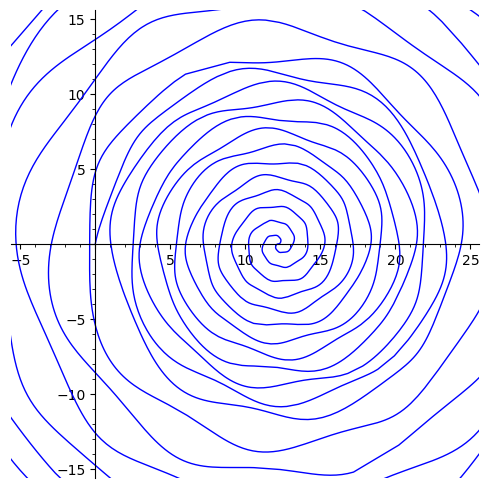
\includegraphics[height=17cm]{f2.png}

\Problem
Let's define $\log_5$ so that $\log_5(5) = 1$
and is continuous at points not on the blue spiral.
What is $\log_5(20)$, symbolically?

\Problem
Consider this Dirichlet problem on a circle:
That is, $u$ is harmonic inside the circle,
continuously extending to the boundary,
and $u(e^{i\theta}) = (2\cos(\theta))^{32}$.
What is $u(0 + 0i)$ symbolically?

\Problem
To evaluate $u(0 + 0i)$ numerically, you can ask your calculator
to compute the numerical integral using the $\int^{[]}_{[]} []$ button.
You can also consider the binomial expansion
\[
    (2\cos(\theta))^{32} = (e^{i\theta} + e^{-i\theta})^{32}
    = \sum_{k=0}^{32} \binom{32}{k} e^{i\theta(32 - 2k)}
\]
and integrate term-by-term.
What is the integer closest to $u(0 + 0i)$?

\Problem
Let's solve another Dirichlet problem:
This time, the initial values are put on the lines $y = \alpha|x|$
for some fixed constant $\alpha > 0$.
That is, $u(x, \alpha|x|) = j(x)$ for some function $j$.
What is $u(0 + 1i)$, symbolically?

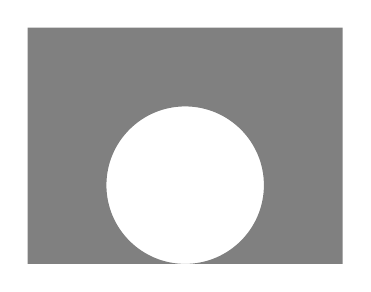
\begin{tikzpicture}
    \fill[gray, even odd rule] (-2, 0) rectangle (2, 3) (0, 1) circle (1);
\end{tikzpicture}
\\[-4cm]

\hangindent=4.5cm \hangafter=-8
\Problem
A circle centered at $2i$ is tangent to the real axis.
Cut away the interior of the circle from the upper half plane.
What is the conformal map from this domain to the upper half plane?
The answer to this question is in the appendix of the textbook.
But if you do not have the textbook with you,
try to think about how to map the boundary---now
a straight line plus a circle---to straight lines.
\\~\\
\Problem
If $f$ and $g$ are holomorphic functions on the entire $\CC$
and $f(n) = g(n)$ for all Gaussian integers $n$,
Does this imply $f = g$ on the entire $\CC$?
Tell me the name of the theorem used or give a counterexample.

\Problem
$u$ is a harmonic function on the half plane $y > -1$.
It also satisfies the property that, for all $z \in \RR$,
$u_{xx}(x, 0) = u_{yy}(x, 0)$.
Show that $u$ is the real part of a holomorphic function $h$
that is defined on the entire $\CC$, not just the half plane.
How are you going to express $h$?
How are you going to show that such $h$ is unique?
Tell me the theorem you are going to use
and the functions it applies to, etc.

\end{document}